\apendice{Especificación de Diseño}
\label{apendice:especificacion_diseno}

\section{Introducción}
\label{sec:c-introduccion}

Este apéndice describe el diseño de la \textit{suite} de monitorización, análisis y visualización desarrollada para Blender, dentro del contexto de los sistemas de interacción 3D y de la analítica de procesos basada en registros de eventos~\cite{bowman2004,vanderalst2016process}. La solución se organiza en dos add-ons complementarios. El primero, \textit{Data Logger 3D}, se ejecuta durante la sesión de modelado y registra eventos, estados y variaciones relevantes en formato CSV. El segundo add-on trabaja de forma posterior sobre esos CSV, valida los datos, calcula métricas estadísticas A1--A17, métricas geométricas y UV, y presenta los resultados mediante paneles y visualizaciones integradas en Blender.

La información de este anexo se ordena desde los elementos más estables del diseño hasta los aspectos más próximos a la interfaz. En primer lugar se define el modelo de datos; después se describe la arquitectura general; a continuación se detallan los dos add-ons; finalmente se documentan las métricas, la interfaz y las decisiones de diseño. Esta organización evita mezclar decisiones de arquitectura con instrucciones de uso o detalles de programación, que quedan desarrollados en los anexos D y E.

\section{Diseño de datos}
\label{sec:c-diseno-datos}

El sistema no utiliza una base de datos relacional. La persistencia de datos se realiza mediante archivos CSV generados por el add-on Data Logger 3D y posteriormente consumidos por el add-on de análisis. Por este motivo, no procede incluir un diagrama entidad-relación ni un modelo relacional clásico. En su lugar, el diseño de datos se documenta mediante la descripción de los campos del CSV y las variables derivadas calculadas durante el análisis.

\subsection{Campos completos del CSV}
\label{subsec:c-campos-csv}


El CSV constituye el contrato de intercambio entre el add-on de captura y el add-on de análisis. El uso de un formato tabular intermedio resulta adecuado para una fase posterior de limpieza, validación y análisis exploratorio de datos~\cite{mckinney2022python,fayyad1996kdd}. Cada fila representa un cambio significativo de la sesión, no una muestra periódica indiferenciada. La generación de filas se basa en la comparación entre un \textit{snapshot} actual y una línea base anterior, de forma que solo se registran deltas cuando se detecta una variación relevante.

\begin{table}[H]
\centering
\scriptsize
\renewcommand{\arraystretch}{1.15}
\begin{tabularx}{\textwidth}{p{3.1cm}p{3.2cm}X}
\toprule
\textbf{Grupo} & \textbf{Campo} & \textbf{Descripción de diseño} \\
\midrule
Identificación & \texttt{SchemaVersion} & Versión del esquema CSV utilizado. En la versión actual toma el valor \texttt{2}. \\
Identificación & \texttt{LoggerVersion} & Versión del add-on \textit{Data Logger 3D} que generó el archivo CSV. Permite relacionar los datos con la versión concreta del software. \\
Identificación & \texttt{SessionID} & Identificador único de la sesión de registro. Permite diferenciar sesiones distintas, incluso cuando pertenecen al mismo usuario. \\
Identificación & \texttt{UserID} & Identificador seudónimo persistente asociado al usuario en el esquema v2. Sustituye al campo heredado \texttt{USER\_ID} del esquema v1 y no almacena el nombre real del usuario. \\
Tiempo & \texttt{TimeStamp} & Marca temporal absoluta utilizada para ordenar registros. \\
Tiempo & \texttt{Minute}, \texttt{Second} & Tiempo relativo desde el inicio de la captura. Facilita el análisis temporal de la sesión. \\
Vista del usuario & \texttt{UserX}, \texttt{UserY}, \texttt{UserZ} & Posición estimada de la cámara o vista 3D del usuario. \\
Escena & \texttt{SceneRadius} & Radio aproximado de la escena calculado a partir de objetos de tipo malla. \\
Objeto activo & \texttt{ObjX}, \texttt{ObjY}, \texttt{ObjZ} & Centro del objeto activo en coordenadas de mundo. \\
Objeto activo & \texttt{ObjRadius} & Radio aproximado del objeto activo a partir de su caja envolvente. \\
Deltas espaciales & \texttt{ObjDeltaX}, \texttt{ObjDeltaY}, \texttt{ObjDeltaZ} & Variación espacial del objeto activo respecto al estado anterior. \\
Deltas espaciales & \texttt{ObjDeltaRadius} & Cambio del radio del objeto activo. Se utiliza como indicio de transformación o escala. \\
Topología & \texttt{VertexDelta} & Variación en el número de vértices. \\
Topología & \texttt{NgonDelta} & Variación en el número de caras con más de cuatro lados. \\
Topología & \texttt{TriDelta} & Variación en el número de triángulos. \\
Topología & \texttt{NormalDelta} & Variación de normales potencialmente invertidas. \\
Modo & \texttt{ObjModeState} & Indica si el contexto se encuentra en \textit{Object Mode}. \\
Modo & \texttt{EditModeState} & Indica si el contexto se encuentra en \textit{Edit Mode}. \\
Modo & \texttt{ModeChanged} & Marca transiciones entre modos de trabajo. \\
UV & \texttt{UV} & Marca eventos o cambios detectados en coordenadas UV. \\
Escena & \texttt{ObjectDelta} & Cambio en el número de objetos de la escena. \\
Escena & \texttt{ModifierDelta} & Cambio en el número total de modificadores. \\
Operadores & \texttt{CtrlV}, \texttt{ShiftD}, \texttt{AltD}, \texttt{Merge} & Banderas de operadores relevantes para el proceso de modelado. \\
Visualización & \texttt{Occlusion} & Estado asociado a modos de visualización como \textit{wireframe} o \textit{x-ray}. \\
\bottomrule
\end{tabularx}
\caption{Campos completos del CSV utilizado como formato intermedio entre captura y análisis.}
\label{tab:c-campos-csv}
\end{table}

\subsection{Compatibilidad entre versiones del esquema CSV}
\label{subsec:c-compatibilidad-csv}

Durante el desarrollo del proyecto el formato CSV ha evolucionado desde una primera versión funcional hasta un esquema más estructurado y versionado. En la versión inicial, denominada esquema v1, el identificador seudónimo del usuario se almacenaba en el campo \texttt{USER\_ID}. Este formato permitía asociar registros a un mismo usuario, pero no incluía información explícita sobre la versión del esquema, la versión del logger ni la sesión concreta de registro.

En la versión actual, denominada esquema v2, se introduce una cabecera más completa formada, entre otros, por los campos \texttt{SchemaVersion}, \texttt{LoggerVersion}, \texttt{SessionID} y \texttt{UserID}. En este nuevo esquema, el campo \texttt{UserID} sustituye a \texttt{USER\_ID} como identificador seudónimo del usuario. La diferencia de nombre no implica dos identificadores distintos, sino una evolución del contrato de datos entre \textit{Data Logger 3D} y \textit{Analysis 3D}.

Para mantener compatibilidad con registros generados por versiones anteriores del logger, \textit{Analysis 3D} detecta automáticamente si el CSV cargado sigue el esquema v1 o v2. En caso de cargar un archivo v1, el sistema normaliza internamente sus campos al formato actual, de forma que los datos antiguos puedan analizarse sin intervención manual.

\begin{table}[H]
\centering
\small
\renewcommand{\arraystretch}{1.15}
\begin{tabularx}{\textwidth}{p{2.5cm}p{3.5cm}X}
\toprule
\textbf{Versión} & \textbf{Campo de usuario} & \textbf{Descripción} \\
\midrule
v1 & \texttt{USER\_ID} & Campo heredado utilizado en las primeras versiones del logger para identificar de forma seudónima al usuario. No incluía campos explícitos de versionado del esquema. \\
v2 & \texttt{UserID} & Campo actual del esquema CSV. Se utiliza junto con \texttt{SchemaVersion}, \texttt{LoggerVersion} y \texttt{SessionID} para mejorar la trazabilidad de los registros. \\
\bottomrule
\end{tabularx}
\caption{Diferencias entre los campos de identificación de usuario en las versiones del esquema CSV.}
\label{tab:csv-userid-v1-v2}
\end{table}

\subsection{Variables derivadas del análisis}
\label{subsec:c-variables-derivadas}

El add-on de análisis conserva los datos originales y calcula variables derivadas únicamente en memoria. Estas variables permiten obtener métricas agregadas sin alterar el CSV fuente. Las derivaciones principales son: duración total de sesión, diferencias temporales entre filas, velocidad de movimiento de la vista, distancia a objeto, actividad de edición por fila, cambios de modo, eventos UV, evolución de vértices, evolución de errores topológicos, métricas de \textit{Object Mode}, métricas geométricas del objeto activo y métricas UV.

\begin{table}[H]
\centering
\scriptsize
\renewcommand{\arraystretch}{1.15}
\begin{tabularx}{\textwidth}{p{4cm}X}
\toprule
\textbf{Variable derivada} & \textbf{Origen y finalidad} \\
\midrule
Tiempo transcurrido & Se obtiene a partir de \texttt{TimeStamp} o de \texttt{Minute}/\texttt{Second}; permite calcular duración y pausas. \\
Velocidad de vista & Se calcula con posiciones \texttt{UserX}, \texttt{UserY}, \texttt{UserZ} y diferencias temporales; sirve para métricas espaciales. \\
Distancia a objeto & Relaciona la posición de la vista con \texttt{ObjX}, \texttt{ObjY}, \texttt{ObjZ}; permite estudiar proximidad. \\
Actividad de edición & Agrega deltas topológicos, cambios de objeto, modificadores, UV y operadores; permite distinguir actividad e inactividad. \\
Tamaño local del objeto & Se aproxima con dimensiones, escala, tamaño disponible o \texttt{ObjRadius}; se usa en métricas de relación espacial. \\
Distribuciones por métrica & Generan mínimo, máximo, media y cuartiles solo cuando la métrica tiene distribución significativa. \\
\bottomrule
\end{tabularx}
\caption{Variables derivadas principales calculadas por el add-on de análisis.}
\label{tab:c-variables-derivadas}
\end{table}

\section{Diseño arquitectónico}
\label{sec:c-diseno-arquitectonico}

La arquitectura se estructura en dos add-ons conectados mediante un CSV intermedio. Esta división responde a criterios clásicos de modularidad y separación de responsabilidades, donde cada componente encapsula una función concreta del sistema~\cite{parnas1972criteria,gamma1994}. Esta separación permite que la captura sea ligera y que el análisis se ejecute bajo demanda. El primer add-on no necesita conocer las métricas finales; el segundo add-on no necesita intervenir durante la sesión de modelado. La Figura~\ref{fig:c-flujo-arquitectura} resume esta relación entre captura, exportación, análisis y visualización.

\begin{figure}[H]
    \centering
    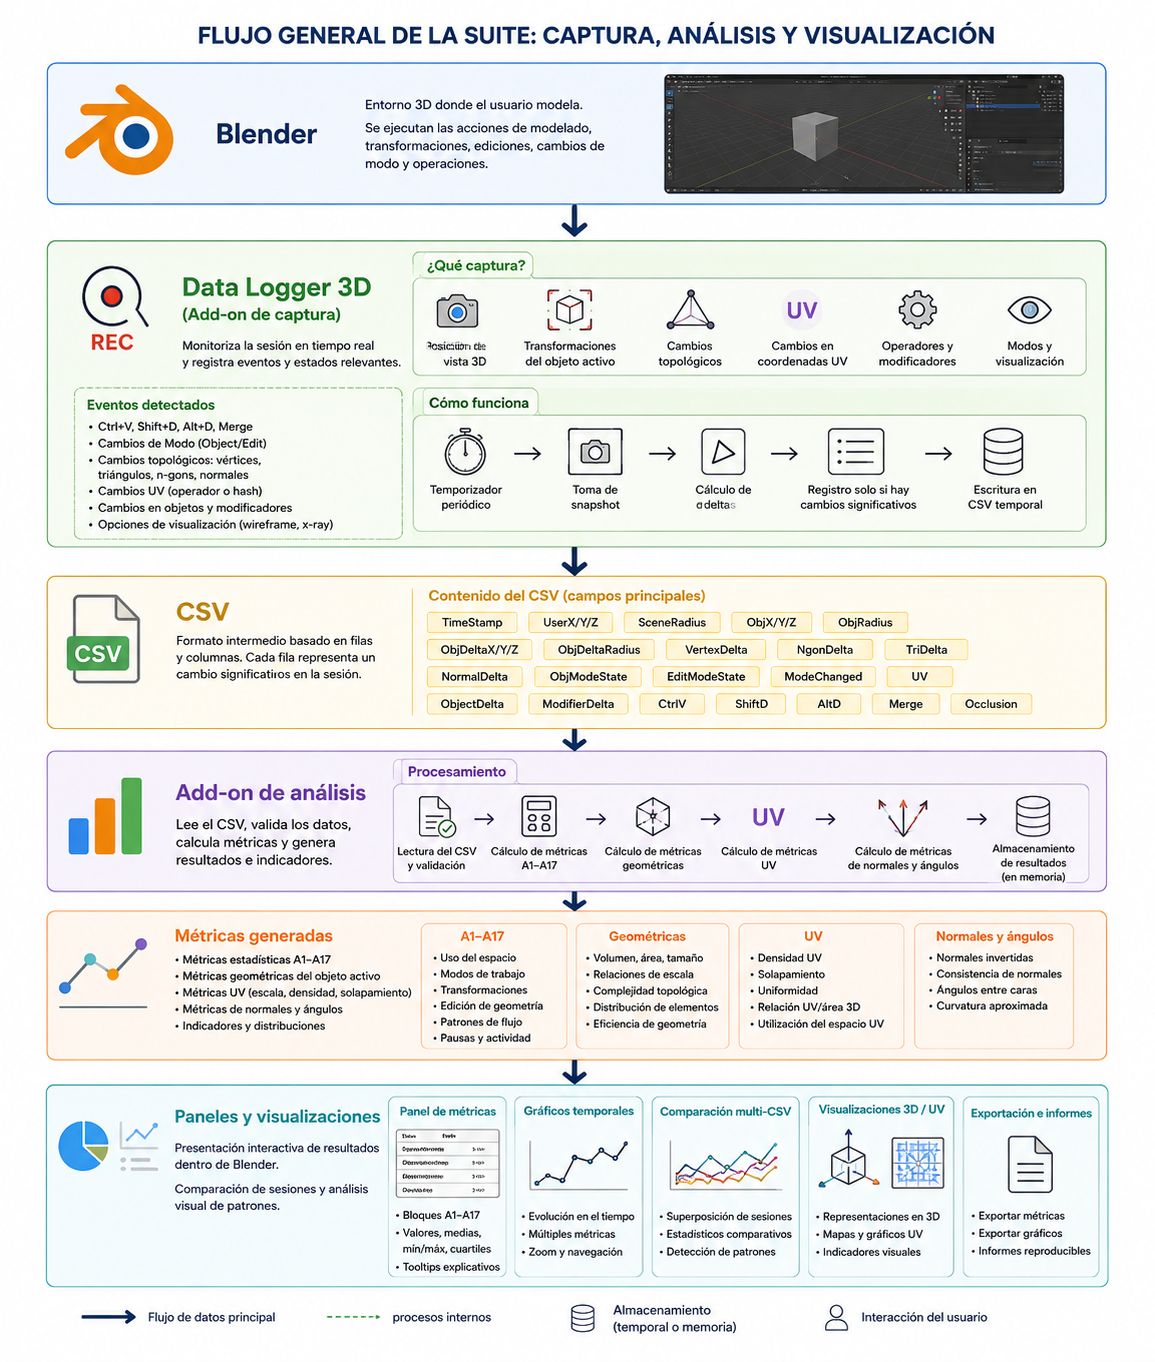
\includegraphics[width=0.95\textwidth]{diagramas/flujo_suite.png}
    \caption{Flujo general de la \textit{suite}: captura, exportación CSV, análisis de métricas y visualización en Blender.}
    \label{fig:c-flujo-arquitectura}
    {\footnotesize \textit{Nota. Figura elaborada por la autora con asistencia de ChatGPT.}}
\end{figure}

Como se observa en la Figura~\ref{fig:c-flujo-arquitectura}, el CSV actúa como punto de unión entre los dos add-ons. Esta decisión evita acoplar directamente el proceso de captura con el cálculo de métricas y permite revisar los datos de forma independiente antes del análisis.

\begin{table}[H]
\centering
\scriptsize
\renewcommand{\arraystretch}{1.15}
\begin{tabularx}{\textwidth}{p{3.5cm}X}
\toprule
\textbf{Componente} & \textbf{Responsabilidad de diseño} \\
\midrule
\textit{Data Logger 3D} & Captura estados, operadores y deltas durante el modelado. Debe ser no intrusivo y robusto ante cambios de contexto. \\
CSV intermedio & Actúa como contrato estable, auditable y portable entre captura y análisis. \\
Add-on de análisis & Lee, valida, calcula métricas y genera visualizaciones sin modificar los datos originales. \\
Paneles de Blender & Proporcionan acceso a captura, exportación, selección de CSV, cálculo e interpretación de resultados. \\
\bottomrule
\end{tabularx}
\caption{Responsabilidades principales de la arquitectura.}
\label{tab:c-arquitectura-componentes}
\end{table}

\subsection{Modelo de componentes y dependencias internas}
\label{subsec:c-modelo-componentes}

El diseño arquitectónico no se limita a la existencia de dos add-ons, sino que define una separación de responsabilidades entre captura, persistencia, análisis, cálculo e interfaz. Esta distribución se representa en la Figura~\ref{fig:c-arquitectura-componentes}, donde se observa cómo cada componente tiene una función delimitada dentro de la \textit{suite}.

\begin{figure}[H]
    \centering
    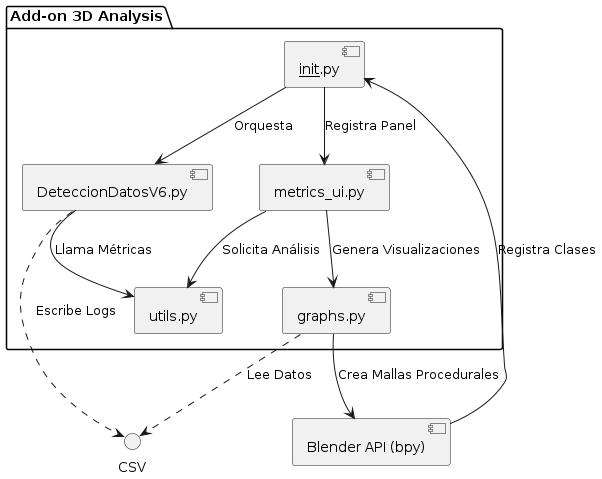
\includegraphics[width=0.9\textwidth]{diagramas/arquitectura_componentes.png}
    \caption{Organización general de componentes y comunicación entre el logger, el CSV y el add-on de análisis.}
    \label{fig:c-arquitectura-componentes}
\end{figure}

La Figura~\ref{fig:c-arquitectura-componentes} permite identificar las dependencias principales del sistema. El logger depende del contexto de Blender para capturar cambios, pero no depende de los módulos de análisis. A su vez, el add-on de análisis depende del CSV exportado y de los objetos seleccionados en Blender cuando se calculan métricas de malla, pero no necesita intervenir durante la captura.

\begin{table}[H]
\centering
\scriptsize
\renewcommand{\arraystretch}{1.15}
\begin{tabularx}{\textwidth}{p{3.4cm}p{4.3cm}X}
\toprule
\textbf{Capa de diseño} & \textbf{Componentes asociados} & \textbf{Criterio de separación} \\
\midrule
Captura & \textit{Data Logger 3D}, temporizador, handlers, operadores & Se ejecuta durante el modelado y debe ser ligera, por lo que solo registra cambios significativos. \\
\midrule
Persistencia & CSV temporal, bloque interno \texttt{data\_log\_internal.csv}, exportación & Conserva los datos en un formato estable y revisable, independiente de la interfaz de análisis. \\
\midrule
Procesamiento & Lectura, validación, métricas A1--A17, métricas geométricas y UV & Trabaja bajo demanda y puede realizar cálculos más costosos sin afectar a la captura. \\
\midrule
Presentación & Paneles, pestañas, tooltips, gráficos y visualizaciones 3D & Muestra resultados al usuario sin modificar los datos originales ni mezclar cálculo con interfaz. \\
\bottomrule
\end{tabularx}
\caption{Capas lógicas utilizadas para organizar el diseño de la suite.}
\label{tab:c-capas-diseno}
\end{table}

\subsection{Diseño modular del código}
\label{subsec:c-diseno-modular-codigo}

La organización del código responde a un criterio de bajo acoplamiento, siguiendo el principio de descomposición modular para reducir dependencias internas y facilitar el mantenimiento~\cite{parnas1972criteria,pressman2005}. El primer add-on se mantiene como un módulo único porque su responsabilidad principal es la captura en tiempo real. En cambio, el add-on de análisis se divide en módulos especializados para separar lectura de datos, cálculo de métricas, generación de gráficos, propiedades de interfaz y operadores de usuario. Esta separación se resume en la Figura~\ref{fig:c-estructura-modular-codigo}.

\begin{figure}[H]
    \centering
    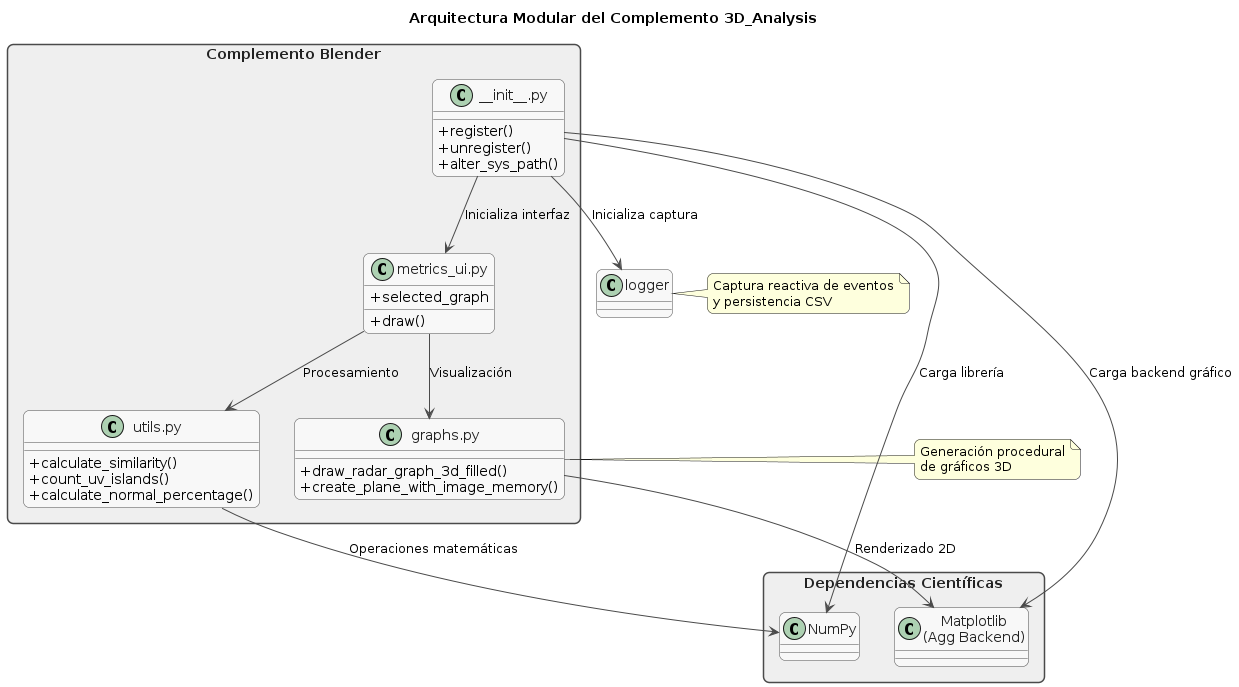
\includegraphics[width=0.9\textwidth]{diagramas/estructura_modular.png}
    \caption{Estructura modular del código y separación entre lógica de cálculo, interfaz y visualización.}
    \label{fig:c-estructura-modular-codigo}
\end{figure}

Como muestra la Figura~\ref{fig:c-estructura-modular-codigo}, los módulos de cálculo se mantienen separados de los paneles de interfaz. Esta decisión facilita la depuración de métricas, la sustitución de funciones de cálculo y la incorporación de nuevas visualizaciones sin modificar la lectura del CSV ni la estructura principal del add-on.

\subsection{Interacción entre captura, análisis e interfaz}
\label{subsec:c-interaccion-captura-analisis}

El flujo de interacción se diseña como una secuencia cerrada: primero se captura, después se persiste, posteriormente se analiza y finalmente se visualiza. La comunicación entre fases se realiza mediante artefactos concretos, principalmente el CSV y las estructuras de resultados generadas en memoria por el add-on de análisis. La Figura~\ref{fig:c-diagrama-secuencia-suite} representa esta interacción completa entre Blender, el logger, el CSV y el add-on de análisis.

\begin{figure}[H]
    \centering
    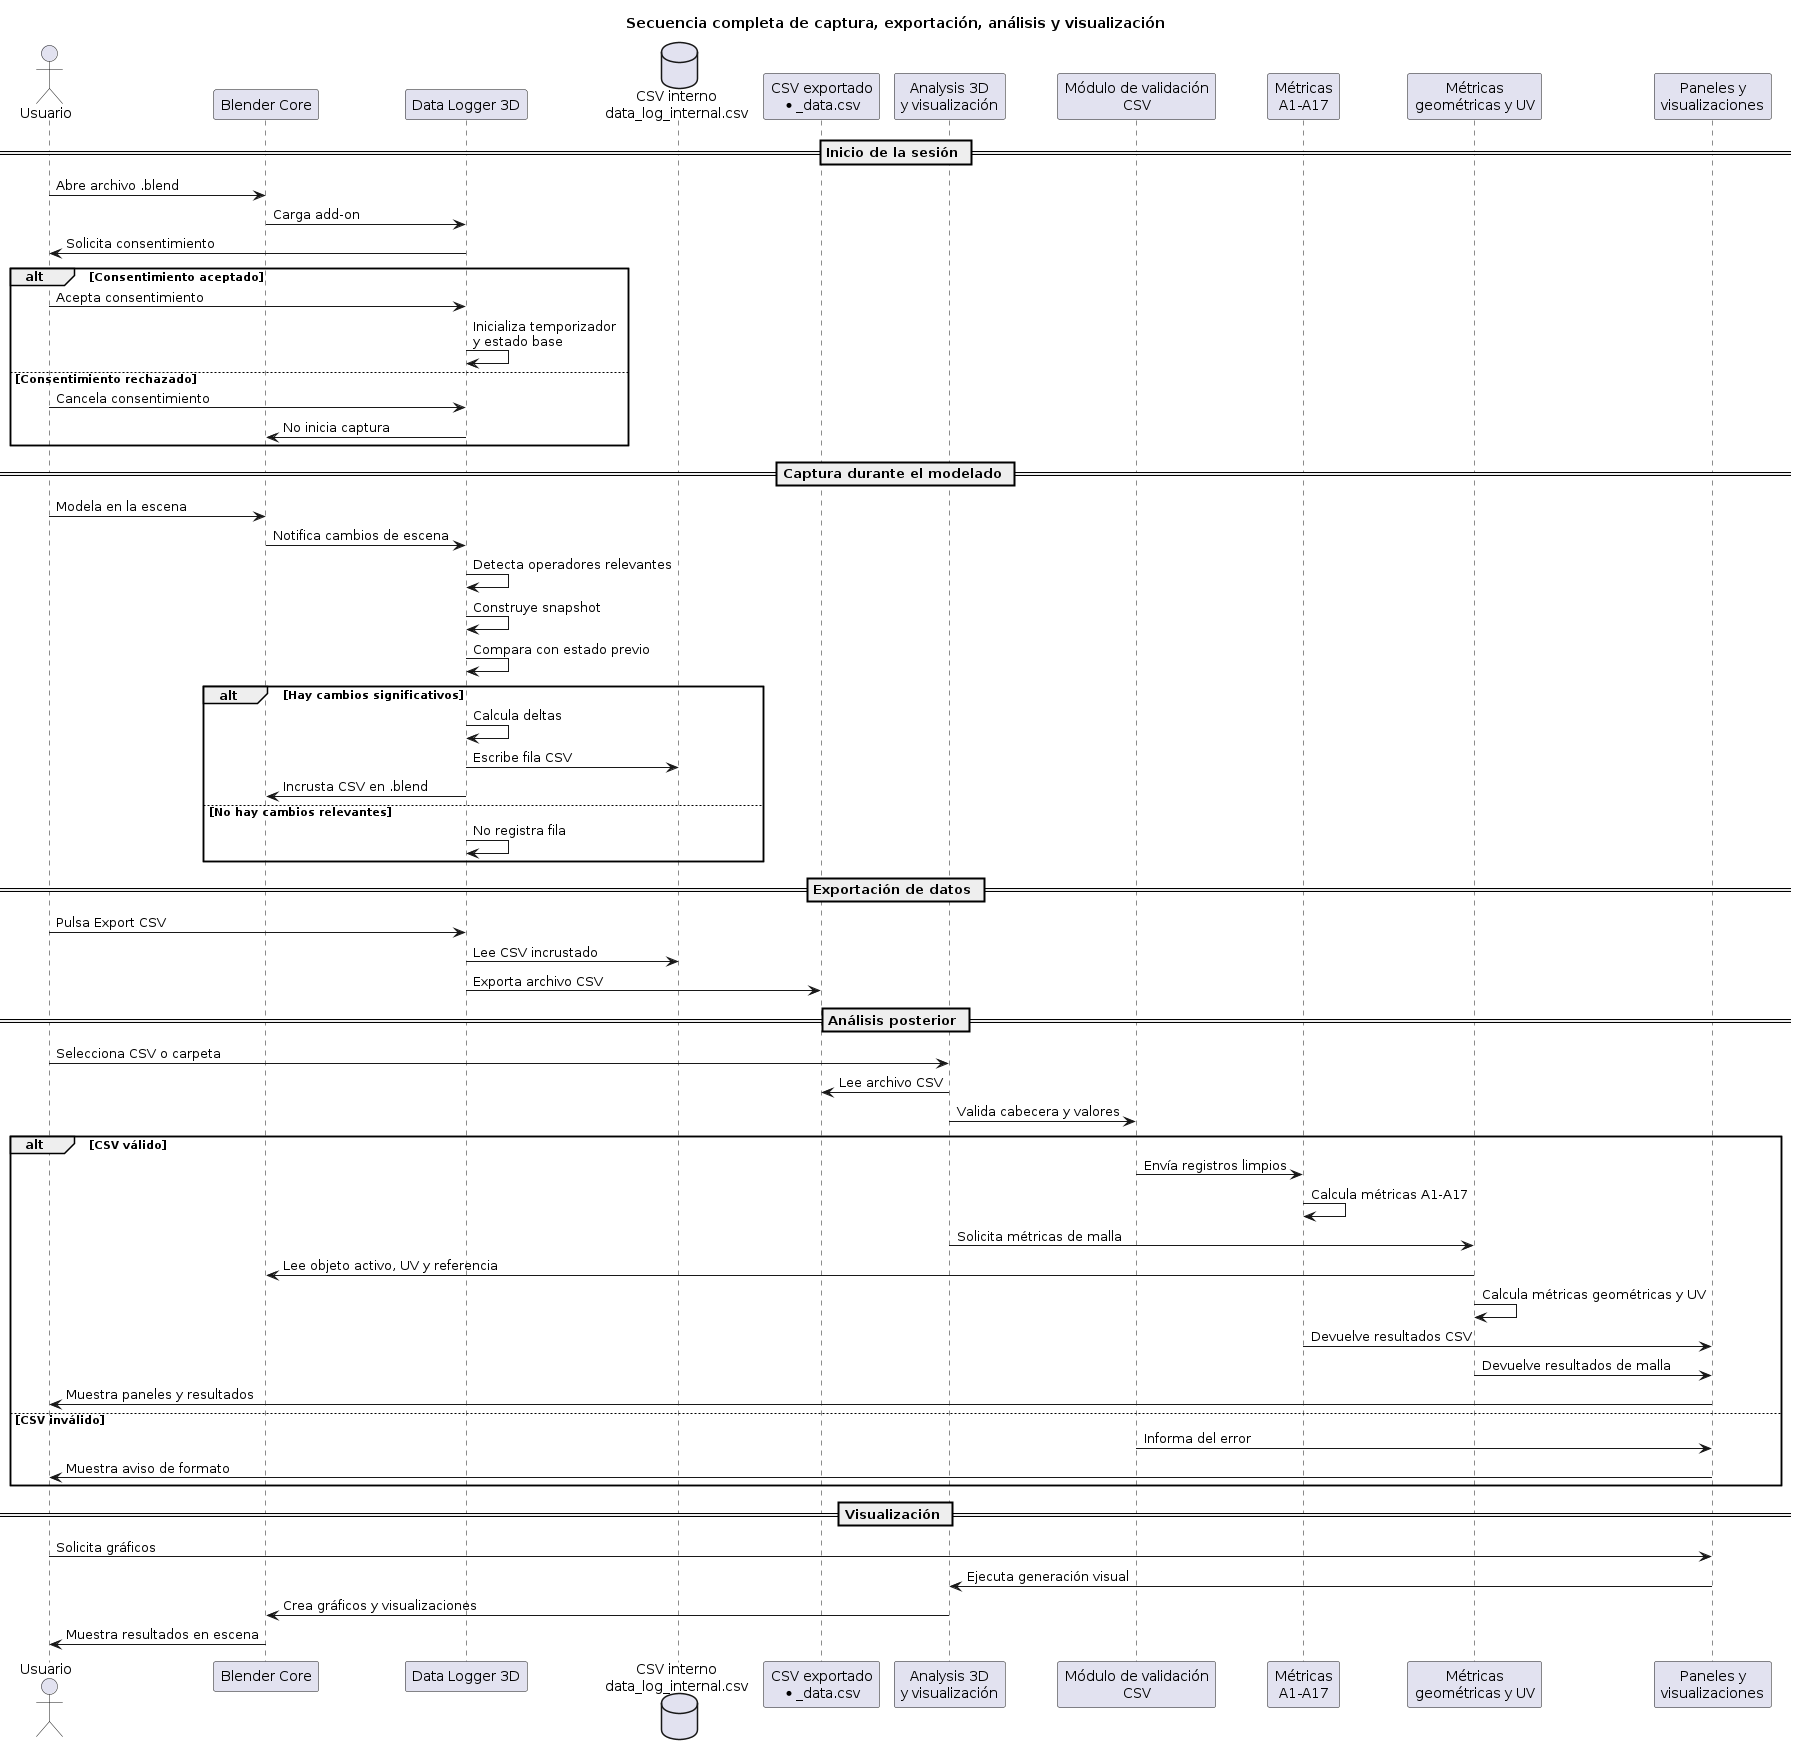
\includegraphics[width=0.9\textwidth]{diagramas/anexos_flujo.png}
    \caption{Secuencia de interacción completa entre Blender, el add-on Data Logger 3D, el CSV intermedio y el add-on de análisis y visualización.}
    \label{fig:c-diagrama-secuencia-suite}
\end{figure}

En la Figura~\ref{fig:c-diagrama-secuencia-suite} se observa que el usuario no interactúa directamente con las funciones internas de cálculo. La interfaz lanza operadores de Blender, estos operadores invocan la lógica correspondiente y los resultados se devuelven al panel o a la escena como elementos visuales. Este diseño evita que el usuario tenga que manipular archivos internos o estructuras de datos intermedias.

\section{Diseño del primer add-on: Data Logger 3D}
\label{sec:c-diseno-logger}

El primer add-on se encarga de registrar los cambios relevantes que se producen durante la sesión de modelado. Su diseño se relaciona con los enfoques de análisis de procesos basados en eventos, donde las acciones se registran para reconstruir posteriormente el comportamiento observado~\cite{vanderalst2016process}. Su prioridad es registrar información útil sin ralentizar la interacción del usuario. Para ello, se organizan varios subsistemas que comparten un estado global mínimo.

\begin{table}[H]
\centering
\scriptsize
\renewcommand{\arraystretch}{1.15}
\begin{tabularx}{\textwidth}{p{3.6cm}X}
\toprule
\textbf{Subsistema} & \textbf{Criterio de diseño} \\
\midrule
Estado global & Mantiene temporizador, línea base anterior, modo previo, objeto activo previo, hash UV y banderas de operadores. \\
Captura espacial & Obtiene posición de la vista, centro del objeto activo, radio del objeto y radio de escena mediante matrices y cajas envolventes. \\
Captura topológica & Cuenta vértices, triángulos, n-gons y normales potencialmente invertidas. Usa \texttt{bmesh} cuando el objeto está en edición. \\
Operadores & Detecta \texttt{Ctrl+V}, \texttt{Shift+D}, \texttt{Alt+D} y \texttt{Merge} mediante operadores recientes, normalización de identificadores y banderas. \\
UV & Combina operadores UV conocidos con un hash global de coordenadas UV para detectar cambios que no aparecen en contadores topológicos. \\
Snapshots y deltas & Compara firma actual y firma previa; solo registra si existe cambio relevante o una bandera forzada. \\
Temporizador & Ejecuta la comprobación de forma periódica y devuelve un intervalo corto mientras el logger está activo. \\
Consentimiento & Exige aceptación antes de iniciar la captura y recuerda el estado mediante un bloque de texto interno. \\
Paneles & Ofrecen control básico de inicio/parada, exportación y depuración. \\
Exportación & Incrusta el CSV en el archivo \texttt{.blend} y permite exportarlo junto al proyecto. \\
\bottomrule
\end{tabularx}
\caption{Diseño interno del add-on Data Logger 3D.}
\label{tab:c-diseno-logger}
\end{table}

El diseño del logger puede entenderse como una máquina de estados sencilla. Mientras el logger está detenido no se escriben filas. Cuando el usuario acepta el consentimiento, el sistema inicializa la línea base, activa el temporizador y pasa al estado de captura. En cada ciclo se compara la escena actual con el \textit{snapshot} anterior; si no existen cambios, no se escribe nada, y si existe una variación relevante, se genera una fila CSV y se actualiza la línea base.

El funcionamiento del logger se divide en dos fases principales. La primera corresponde a la detección de cambios durante la sesión de modelado, representada en la Figura~\ref{fig:c-flujo-interno-logger}. La segunda corresponde a la persistencia y exportación del CSV generado, representada en la Figura~\ref{fig:c-exportacion-csv-logger}. Esta separación permite distinguir entre el registro automático de la actividad y la obtención posterior de un archivo CSV externo para el análisis.

\begin{figure}[H]
    \centering
    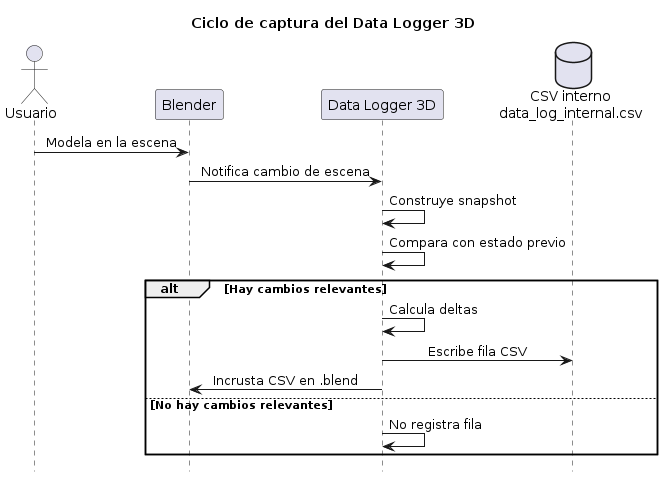
\includegraphics[width=0.9\textwidth]{diagramas/anexos_data_logger.png}
    \caption{Flujo interno de detección de cambios del Data Logger 3D durante una sesión de modelado.}
    \label{fig:c-flujo-interno-logger}
\end{figure}

La Figura~\ref{fig:c-flujo-interno-logger} muestra la fase de observación y detección. En esta parte se obtiene el estado actual de Blender, se identifican datos espaciales, topológicos, de modo, operadores y UV, y se construye una representación resumida de la sesión. Esta información se compara con la línea base anterior para decidir si existe un cambio suficientemente relevante como para registrar una nueva fila.

\begin{figure}[H]
    \centering
    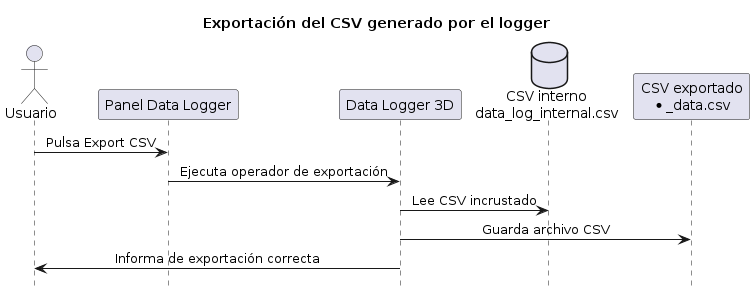
\includegraphics[width=0.9\textwidth]{diagramas/anexos_csv.png}
    \caption{Flujo de persistencia y exportación del CSV generado por el Data Logger 3D.}
    \label{fig:c-exportacion-csv-logger}
\end{figure}

La Figura~\ref{fig:c-exportacion-csv-logger} representa la fase de persistencia y exportación. Durante la captura, los registros se conservan como CSV interno asociado al archivo \texttt{.blend}. Cuando el usuario solicita la exportación, el add-on recupera ese contenido interno y genera un archivo CSV externo en la carpeta del proyecto. Este archivo actúa como entrada para el add-on de análisis y permite revisar los datos fuera de Blender si fuera necesario.

A partir de las fases mostradas en las Figuras~\ref{fig:c-flujo-interno-logger} y~\ref{fig:c-exportacion-csv-logger}, el comportamiento del logger puede resumirse como una máquina de estados sencilla. La Tabla~\ref{tab:c-estados-logger} recoge los estados principales y las acciones asociadas a cada transición.

\begin{table}[H]
\centering
\scriptsize
\renewcommand{\arraystretch}{1.15}
\begin{tabularx}{\textwidth}{p{3cm}p{4cm}X}
\toprule
\textbf{Estado} & \textbf{Entrada o evento} & \textbf{Acción de diseño} \\
\midrule
Detenido & Add-on cargado sin captura activa & No se escriben registros y el panel solo muestra controles de inicio o consentimiento. \\
\midrule
Inicialización & Consentimiento aceptado o inicio manual & Se crea o restaura el CSV, se calcula el primer snapshot y se fija la línea base. \\
\midrule
Captura & Ciclo del temporizador & Se comparan estado actual y estado previo, se detectan operadores y se evalúa si procede registrar. \\
\midrule
Persistencia & Cambio relevante detectado & Se escribe una fila, se eliminan duplicados y se incrusta el CSV en el archivo \texttt{.blend}. \\
\midrule
Exportación & Acción del usuario & Se vuelca el CSV incrustado a un archivo externo junto al proyecto. \\
\bottomrule
\end{tabularx}
\caption{Estados principales del diseño de ejecución del Data Logger 3D.}
\label{tab:c-estados-logger}
\end{table}

\section{Diseño del segundo add-on: análisis y visualización}
\label{sec:c-diseno-analisis}

El segundo add-on se diseña como una capa de procesamiento posterior. Esta decisión aproxima la herramienta a un flujo de análisis exploratorio: primero se validan los datos, después se calculan métricas y finalmente se generan representaciones visuales interpretables~\cite{fayyad1996kdd,munzner2014visualization}. La lectura CSV, la validación, el cálculo estadístico, el cálculo geométrico y la interfaz se mantienen separados para reducir dependencias cruzadas y facilitar el mantenimiento.

\begin{table}[H]
\centering
\scriptsize
\renewcommand{\arraystretch}{1.15}
\begin{tabularx}{\textwidth}{p{3.7cm}X}
\toprule
\textbf{Bloque} & \textbf{Responsabilidad de diseño} \\
\midrule
Lectura CSV & Localiza archivos individuales o carpetas y convierte las filas a estructuras procesables. \\
Validación & Comprueba cabeceras, valores numéricos, ausencia de infinitos y tratamiento de datos no disponibles. \\
Cálculo estadístico & Calcula A1--A17 a partir de posiciones, tiempos, deltas, modos y operadores. \\
Cálculo geométrico & Evalúa propiedades de malla, similitud, distancia de Hausdorff, normales, ángulos y topología. \\
Cálculo UV & Calcula área UV, islas, estiramiento y densidad de texeles, entendida como la relación entre resolución de textura y superficie del modelo. \\
Visualización & Genera gráficos, objetos procedurales y representaciones comparativas dentro de Blender. \\
Interfaz & Presenta resultados en paneles compactos, con etiquetas breves y tooltips explicativos. \\
\bottomrule
\end{tabularx}
\caption{Diseño interno del add-on de análisis y visualización.}
\label{tab:c-diseno-analisis}
\end{table}

El diseño del add-on de análisis sigue una arquitectura por capas. Las rutas seleccionadas por el usuario se gestionan desde la interfaz, la lectura transforma los CSV en estructuras internas, la validación filtra valores no válidos y los módulos de cálculo generan resultados independientes de la presentación. Finalmente, la capa de interfaz decide si esos resultados se muestran como texto, bloques de métricas, gráficos o visualizaciones en la escena.

La secuencia de funcionamiento del segundo add-on se muestra en la Figura~\ref{fig:c-secuencia-analisis-visualizacion}. A diferencia del logger, este componente se ejecuta bajo demanda: el usuario selecciona un CSV o una carpeta, el sistema valida los datos y posteriormente distribuye la información entre los módulos de cálculo y visualización.

\begin{figure}[H]
    \centering
    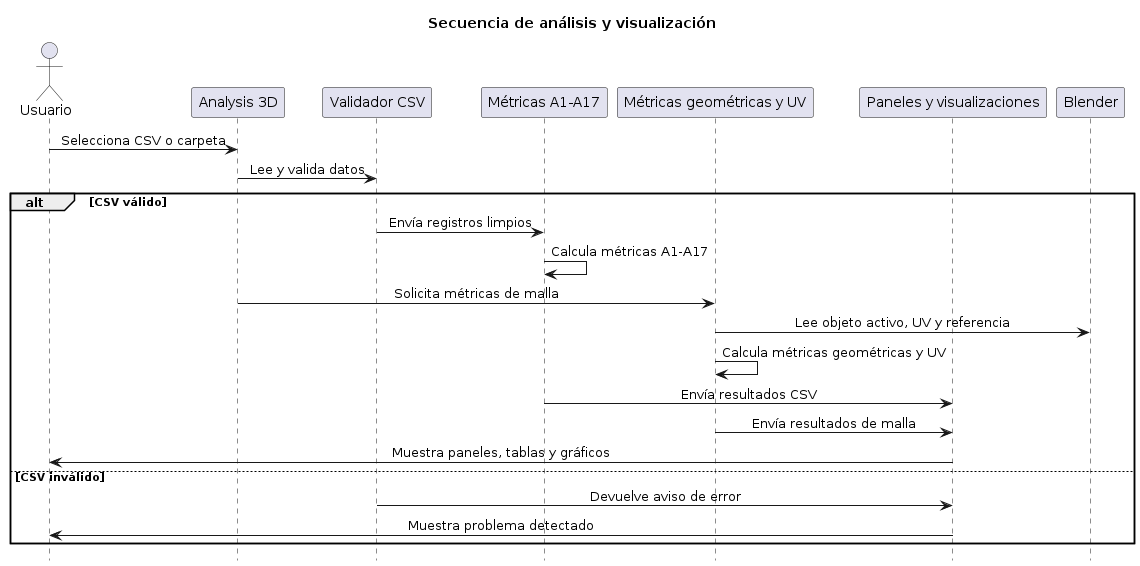
\includegraphics[width=0.9\textwidth]{diagramas/anexos_analisis1.png}
    \caption{Secuencia de análisis, cálculo de métricas y visualización de resultados en el segundo add-on.}
    \label{fig:c-secuencia-analisis-visualizacion}
\end{figure}

Como se observa en la Figura~\ref{fig:c-secuencia-analisis-visualizacion}, el cálculo estadístico y el cálculo de métricas de malla se mantienen separados. Esta separación permite analizar sesiones completas a partir del CSV y, al mismo tiempo, calcular métricas geométricas o UV sobre el objeto activo de Blender cuando el usuario lo solicita.

La Tabla~\ref{tab:c-flujo-modulos-analisis} resume esta transformación desde las entradas de usuario hasta las salidas generadas por el add-on. De este modo se documenta qué recibe cada módulo lógico y qué resultado produce dentro del diseño general.

\begin{table}[H]
\centering
\scriptsize
\renewcommand{\arraystretch}{1.15}
\begin{tabularx}{\textwidth}{p{3.6cm}p{4cm}X}
\toprule
\textbf{Módulo lógico} & \textbf{Entrada} & \textbf{Salida de diseño} \\
\midrule
Lectura CSV & Ruta de archivo o carpeta & Lista de registros normalizados para cálculo. \\
\midrule
Validación & Registros leídos & Datos numéricos seguros, sin valores infinitos ni campos incompatibles. \\
\midrule
Métricas A1--A17 & Datos temporales, espaciales y de actividad & Diccionario de métricas estadísticas y distribuciones. \\
\midrule
Métricas de malla & Objeto activo y, si procede, referencia & Valores geométricos, UV, similitud y distancias. \\
\midrule
Visualización & Resultados calculados & Paneles, gráficos 2D, forest plot, radar y objetos gráficos en Blender. \\
\bottomrule
\end{tabularx}
\caption{Transformación de entradas y salidas en el diseño del add-on de análisis.}
\label{tab:c-flujo-modulos-analisis}
\end{table}

\section{Diseño procedimental}
\label{sec:c-diseno-procedimental}

El procedimiento general se divide en captura, persistencia, análisis y visualización. Esta secuencia ya se ha representado a nivel arquitectónico en la Figura~\ref{fig:c-flujo-arquitectura} y a nivel de componentes en la Figura~\ref{fig:c-arquitectura-componentes}. En este apartado se recoge el mismo flujo de forma operativa, indicando el orden lógico de ejecución.

\begin{enumerate}
    \item Se abre Blender y se activa el add-on \textit{Data Logger 3D}.
    \item El sistema comprueba Auto Run y solicita consentimiento si procede.
    \item Se inicializa o restaura el CSV asociado a la sesión.
    \item El temporizador construye snapshots y detecta cambios significativos.
    \item Las filas se escriben, se depuran duplicados y se incrustan en el \texttt{.blend}.
    \item El CSV se exporta cuando el usuario lo solicita.
    \item El add-on de análisis lee uno o varios CSV y valida sus datos.
    \item Se calculan métricas A1--A17, métricas geométricas y métricas UV.
    \item Los resultados se presentan en paneles y visualizaciones dentro de Blender.
\end{enumerate}

\section{Diseño de métricas A1--A17}
\label{sec:c-diseno-a1-a17}

Las métricas A1--A17 se organizan por tipología para mejorar su lectura. La interfaz no debe repetir valores equivalentes ni mostrar cuartiles cuando no aportan información interpretativa. Por ello, se agrupan A2--A3 y A6--A9, mientras que A12, A13 y A16 conservan distribución propia.

\begin{table}[H]
\centering
\scriptsize
\renewcommand{\arraystretch}{1.12}
\begin{tabularx}{\textwidth}{p{1.3cm}p{3.8cm}p{2.5cm}X}
\toprule
\textbf{ID} & \textbf{Etiqueta} & \textbf{Tipo} & \textbf{Diseño de presentación} \\
\midrule
A1 & Total time & Temporal & Duración total, sin cuartiles. \\
A2 & Breaks & Temporal & Agrupada con A3 por compartir interpretación temporal. \\
A3 & Breaks by phase & Temporal & Agrupada con A2; resume distribución de pausas por fase. \\
A4 & Movement speed & Spatial & Muestra resumen estadístico de velocidad. \\
A5 & Proximity to object & Spatial & Muestra relación espacial con el objeto activo. \\
A6 & View manipulation & Spatial & Agrupada con A7--A9 para evitar bloques redundantes. \\
A7 & Speed during inactivity & Spatial & Interpretación conjunta con actividad/inactividad. \\
A8 & Speed during activity & Spatial & Comparación frente a velocidad en inactividad. \\
A9 & Distance travelled & Spatial & Completa el bloque de desplazamiento. \\
A10 & Acceleration strategy 1 & Strategy & Bloque independiente de estrategia. \\
A11 & Acceleration strategy 2 & Strategy & Bloque independiente de estrategia. \\
A12 & Vertex evolution & Strategy & Mantiene distribución propia y cuartiles. \\
A13 & Error evolution & Strategy & Mantiene distribución propia y cuartiles. \\
A14 & Object Mode & Strategy & Se etiqueta explícitamente como métrica de \textit{Object Mode}. \\
A15 & UV work & Strategy & Se vincula a eventos o cambios UV. \\
A16 & Mesh evolution & Strategy & Mantiene distribución propia. \\
A17 & Object change delta & Strategy & Resume variaciones de objeto en \textit{Object Mode}. \\
\bottomrule
\end{tabularx}
\caption{Diseño de presentación de las métricas A1--A17.}
\label{tab:c-diseno-a1-a17}
\end{table}

\section{Diseño de métricas geométricas y UV}
\label{sec:c-diseno-geom-uv}

Las métricas geométricas y UV se calculan directamente sobre objetos de Blender. Este bloque se apoya en conceptos habituales de procesamiento de mallas poligonales y comparación geométrica de superficies~\cite{botsch2010polygon,cignoni1998metro}. Su diseño se separa de las métricas CSV porque dependen del estado de la malla, de capas UV y, en algunos casos, de un objeto de referencia.

\begin{table}[H]
\centering
\scriptsize
\renewcommand{\arraystretch}{1.15}
\begin{tabularx}{\textwidth}{p{3.2cm}X}
\toprule
\textbf{Métrica} & \textbf{Diseño de cálculo} \\
\midrule
\texttt{UV area} & Área ocupada en el espacio UV mediante triangulación o fórmula poligonal sobre coordenadas UV. \\
\texttt{UV islands} & Conteo de componentes conexas en el mapa UV. \\
\texttt{UV stretch} & Relación entre proporciones 3D y proporciones UV para estimar deformación. \\
\texttt{UV texel density} & Relación entre área geométrica y área UV para estimar la distribución de resolución de textura sobre el modelo. \\
\texttt{Normal percentage} & Porcentaje de caras con orientación anómala o potencialmente invertida. \\
\texttt{Angle} & Mediana o resumen de ángulos entre caras adyacentes conectadas por aristas. \\
\texttt{Non-quads} & Recuento o porcentaje de caras que no son cuadrangulares. \\
\texttt{Vertex duplicate} & Detección de vértices coincidentes o muy próximos. \\
\texttt{Similarity} & Comparación geométrica y topológica frente a un objeto de referencia. \\
\texttt{Hausdorff distance} & Máxima distancia mínima entre conjuntos de vértices cuando existe referencia válida. \\
\bottomrule
\end{tabularx}
\caption{Diseño de métricas geométricas y UV.}
\label{tab:c-diseno-geom-uv}
\end{table}

\section{Decisiones de diseño relevantes}
\label{sec:c-decisiones-diseno}

\begin{table}[H]
\centering
\scriptsize
\renewcommand{\arraystretch}{1.15}
\begin{tabularx}{\textwidth}{p{4cm}X}
\toprule
\textbf{Decisión} & \textbf{Justificación} \\
\midrule
Separación en dos add-ons & Evita que el análisis pesado interfiera con el modelado y permite evolucionar cada parte por separado. \\
CSV como formato intermedio & Facilita trazabilidad, revisión manual, portabilidad y compatibilidad con herramientas externas. \\
Captura basada en snapshots & Reduce registros redundantes y permite calcular deltas de forma controlada. \\
Uso de \texttt{bmesh} & Permite leer topología y UV con mayor precisión en \textit{Edit Mode}. \\
Hash UV & Detecta cambios de coordenadas UV aunque no cambien los contadores topológicos. \\
Uso de KDTree & Se incorpora en las métricas geométricas que requieren búsquedas de proximidad entre puntos, especialmente en comparaciones entre mallas, siguiendo la idea de búsqueda espacial eficiente propuesta para árboles multidimensionales~\cite{bentley1975kdtree}. Su uso permite reducir el coste de cálculo frente a comparaciones exhaustivas y mejora el rendimiento en modelos con mayor número de vértices. \\
Separación lógica/interfaz & Mejora mantenibilidad y permite probar cálculo y validación sin depender del panel gráfico. \\
Tooltips y bloques compactos & Conservan información contextual sin saturar la interfaz lateral de Blender. \\
\bottomrule
\end{tabularx}
\caption{Decisiones de diseño relevantes de la \textit{suite}.}
\label{tab:c-decisiones-diseno}
\end{table}

\section{Síntesis del diseño}
\label{sec:c-sintesis}

El diseño propuesto combina una fase de captura ligera con una fase de análisis flexible. La estructura de datos CSV actúa como punto de unión entre los dos add-ons, mientras que la separación de responsabilidades permite ampliar operadores, métricas o visualizaciones sin modificar todo el sistema. Esta organización proporciona una base técnica coherente para la documentación de programación del anexo D y para las instrucciones de uso del anexo E.